\section{Eruptive Solar Flares}
\subsection{An Introduction to the Standard Eruptive Flare Model} 
standard solar flare model
cartoon
\subsection{Observing Solar Flares}
a bit about the the spacecraft and instrumentation providing the data for my research. Make sure to explain abbreviations
\subsubsection{Solar Atmosphere}
a bit about observing different layers of the atmosphere in different wavelengths...how do we know the altitudes of the emission?
can use modified solar atmosphere section (from old report)....rewrite pressure scale height...i.e,energy moving through the atmosphere has to traverse 9 pressure scale heights...what that means
\subsection{Magnetohydrodynamics of Solar Flares}
mhd maths and explanation..and what the induction equation physically means...maybe use a figure!!!
get to grips with the derivation, why is each assumption made?
can use mhd section from old report



%%%%%%%%%%%%%%%%%%%%%%%%%%%%%%%%%%%%%%%%%%%%%%%%%%%%%%%%%%%%%%%%%%%%
%old report content

%%%%%%%%%%%%%%%%%%%%%%Eruptive Flare Model%%%%%%%%%%%%%%%%%%%%%%%%%%
\subsection{Eruptive Flare Model}\label{EFM}
Solar flares are the manifestation of magnetic energy release in the form of electromagnetic radiation spanning a wide range of wavelengths. These events are the most energetic phenomena associated with the Sun, with some of the larger flares releasing $10^{37}$ erg of energy. Flares are classified by the X-ray flux measured by the Geostationary Operational Environmental Satellite (GOES) see the table below.


\begin{tabular}{|c|c|}\label{GOES}
Classification & Peak Flux Range at $1$ to $8\AA$ ($W.m^{-2}$)\\ 
X & $10^{-3}$ - $10^{-4}$\\ 
M & $10^{-4}$ - $10^{-5}$\\ 
C & $10^{-5}$ - $10^{-6}$\\ 
B & $10^{-6}$ - $10^{-7}$\\ 
A & $<10^{-7}$\\  
\end{tabular}


The exact physical process governing the mechanics of solar flares is not known, however, magnetic reconnection is the currently accepted mechanism. Coronal magnetic loops tethered to sunspots of opposing polarity in the photosphere and sub-photosphere are twisted and stressed by movements of active regions across the solar surface. This shearing of the magnetic field, effectively stores energy as magnetic tension which can be released when opposing field lines meet and reconnect. The process of energy conversion is basically a unstable tensioned magnetic field relaxing back to a more stable configuration. As a result stored magnetic energy is converted to radiation, kinetic and thermal energy\citep{1976SoPh...50...85K}.\\
The standard 2D flare model is the culmination of many papers by many authors,\citep{1964NASSP..50..451C, 1966Natur.211..695S, 1974SoPh...34..323H, 1976SoPh...50...85K}, and is still an ongoing area of research that is not well understood. In an active region, a closed magnetic field harbouring a prominence suddenly opens. As a result, plasma flows from the chromosphere to the corona. Because material in the chromosphere is denser than in the corona, flowing plasma experiences a drop in plasma pressure and an increase in magnetic pressure. This leads to reconnection of the open magnetic field lines, forming new loops at lower altitudes. Reconnection causes excess heating at the peaks of newly connected loops which conducts down toward the chromosphere. Also, particles are accelerated by the new magnetic configuration, flowing to the chromosphere. This injection of thermal energy and accelerated particles heats the chromosphere causing HXR footpoints \citep{1995ApJ...455..347A} and UV ribbons \citep{2009A&A...493..241F}. As a result, some chromospheric material evaporates upward into newly created flare loops, whilst some material propagates downward toward the lower chromosphere, known as condensation. The flare loop cools and the process starts again in the next consecutive loop until the unstable magnetic field has relaxed to a state that is closer to it's stable,  potential state. In eruptive flares, energy is released every time a new reconnection of a neighbouring loop occurs, this said to be the reason that flare ribbons move away from each other as the flare evolves. 

White light flares are said to be rare events only associated with the most energetic of solar flares, they occur when flare energy is transported deep into the dense lower atmosphere causing an enhancement in optical wavelengths. It is thought this happens due to an electron beam transporting energy to the lower atmosphere where it's energy dissipates into the dense chromospheric or photospheric material. The collisional thick target model by \cite{1971SoPh...18..489B} says that almost all of the flare energy is carried by the electron beam, therefore, energy dissipated in the lower atmosphere represents a large portion of the flare energy budget. White light enhancement from the lower atmosphere can be explained by either, Balmer \& Paschen continuum emission from the chromosphere caused by hydrogen recombination or direct photospheric heating \citep{2007ASPC..368..417D}.

%%%%%%%%%%%%%%%%%%%%%%Solar Atmosphere%%%%%%%%%%%%%%%%%%%%%%%%%%
\subsection{Solar Atmosphere}\label{ATM}
The solar atmosphere \citep{2003dysu.book.....D, 2004soas.book.....F} is described as having four main components, the corona, transition region, chromosphere and photosphere. The photosphere is the lowest in altitude of the four layers characterised as having an effective temperature $T=5800$K, the photosphere decreases in temperature with radial distance. Due to the assumption that this region emits as a black body the temperature is estimated using Wien's displacement law. Pressure scale height in this part of the atmosphere is $H\sim150$km. The plasma beta in this region is mostly larger than one $\beta >1$ meaning plasma pressure is the dominant force dictating plasma motions, the exception to this exists in sunspots where $\beta<1$ and magnetic pressure is dominant. Dark, lower temperature patches found in active regions of the photosphere, sunspots are regions of intense magnetic field. They are made up of two main parts, the central umbra, surrounded by the slightly less dark penumbra. The umbra hosts magnetic field lines that are tightly packed and pointing radially away from the Sun, whereas the penumbral magnetic field is more horizontal. Other features that are part of the photosphere include granules and super granules (seen only in Doppler images), which are the physical representation of convection currents. Heated plasma rises from below the surface and is seen as the bright central part of the granule, the darker surrounding regions are cooler material sinking back into the interior. The next region of the atmosphere is the chromosphere which is situated above the photosphere. This layer of plasma is a few thousand kilometres (2000-3000km) thick and is optically thin to visible light so is difficult to see against the brightness of the photosphere. The temperature in this layer increases with height and ranges from 4400K at the temperature minimum region to $\sim10^{5}$K at the top, as a result, $\beta$ drops rapidly crossing unity as it does so. The pressure scale height, based on an average isothermal temperature of $2\times10^{4}$ is $H\sim600$km. The dominant emission in this region is H$\alpha$ at $6563\AA$.

\begin{wrapfigure}{R}{0.48\textwidth}\label{solatm}
  \begin{center}
    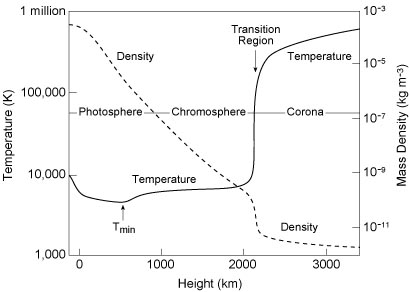
\includegraphics[width=0.45\textwidth]{solar-atm-plot}
  \end{center}
\caption{The temperature of the solar atmosphere decreases from values near 6,000 degrees Kelvin at the visible photosphere to a minimum value of roughly 4,400 degrees Kelvin about 500 kilometers higher up. The temperature increases with height, slowly at first, then extremely rapidly in the narrow transition region, less than 100 kilometers thick, between the chromosphere and corona, from about $10^{4}$K to about $10^{6}$K. (Courtesy of Eugene Avrett, Smithsonian Astrophysical Observatory.) }
\end{wrapfigure}

Through the transition region to the corona and the atmosphere starts to heat considerably to $T\sim10^{7}$K. This region is visible in white light due to Thompson scattering of photospheric light by free electrons and dust in the coronal magnetic field. The plasma beta is less than one through the entire corona meaning magnetic forces dominate and the pressure scale height is approximately $100$Mm.  



